\documentclass[10pt]{article}

%% Urti in laboratorio: quattro esercizi (classe terza, scienze applicate)
%% QR verso Collision Lab (labs.matephis.com/collision-lab), pacchetto qrcode.
%% Copia con soluzioni e indicazioni per il docente:
%%   pdflatex -jobname=esercizi-urti-laboratorio-soluzioni \
%%            "\PassOptionsToPackage{answers}{fancytests}\documentclass[10pt]{article}

%% Urti in laboratorio: quattro esercizi (classe terza, scienze applicate)
%% QR verso Collision Lab (labs.matephis.com/collision-lab), pacchetto qrcode.
%% Copia con soluzioni e indicazioni per il docente:
%%   pdflatex -jobname=esercizi-urti-laboratorio-soluzioni \
%%            "\PassOptionsToPackage{answers}{fancytests}\documentclass[10pt]{article}

%% Urti in laboratorio: quattro esercizi (classe terza, scienze applicate)
%% QR verso Collision Lab (labs.matephis.com/collision-lab), pacchetto qrcode.
%% Copia con soluzioni e indicazioni per il docente:
%%   pdflatex -jobname=esercizi-urti-laboratorio-soluzioni \
%%            "\PassOptionsToPackage{answers}{fancytests}\documentclass[10pt]{article}

%% Urti in laboratorio: quattro esercizi (classe terza, scienze applicate)
%% QR verso Collision Lab (labs.matephis.com/collision-lab), pacchetto qrcode.
%% Copia con soluzioni e indicazioni per il docente:
%%   pdflatex -jobname=esercizi-urti-laboratorio-soluzioni \
%%            "\PassOptionsToPackage{answers}{fancytests}\input{esercizi-urti-laboratorio}"
\usepackage[subject=physics, seed=2026]{fancytests}
\usepackage{lmodern}
\renewcommand*\familydefault{\sfdefault}
\usepackage[T1]{fontenc}
\usepackage{qrcode}
\usepackage{url}

\geometry{a4paper, top=15mm, bottom=15mm, left=17.5mm, right=17.5mm}
\pagestyle{empty}
\linespread{1.12}

\testsetup{labels=boxed, mcq=none, autoclose=false, scores=false}

%% ---------------------------------------------------------------------------
%% QR verso una scena di Collision Lab: testo a sinistra, QR a destra
%% \conqr{frammento dopo #, con \& al posto di &}{testo}
%% ---------------------------------------------------------------------------
\newcommand{\appurl}{https://labs.matephis.com/collision-lab/}
\newcommand{\conqr}[2]{%
  \par\smallskip\noindent
  \begin{minipage}[c]{\dimexpr\linewidth-3.1cm}#2\end{minipage}\hfill
  \begin{minipage}[c]{2.6cm}\centering
    \qrcode[height=2.4cm]{\appurl\##1}\par
    {\scriptsize\color{black!55}Collision Lab}
  \end{minipage}\par\smallskip}

%% grafici di dati: assi a sinistra, griglia fitta, punti senza linee
\pgfplotsset{
  dati/.style={
    axis lines=left, grid=both, grid style={gray!70}, minor grid style={gray!25},
    tick label style={font=\footnotesize}, label style={font=\small},
    legend style={font=\footnotesize, draw=black!40, fill=white},
    legend cell align=left,
  },
  puntoA/.style={only marks, mark=*, mark size=1.6pt, black},
  puntoB/.style={only marks, mark=square*, mark size=1.5pt, black!45},
}

\begin{document}

\noindent{\Large\bfseries Fisica \textperiodcentered{} Urti in laboratorio}\par
\vspace{.4em}\noindent{\color{black!45}\rule{\textwidth}{.4pt}}\par\vspace{.4em}

\noindent Dove c'è un QR, la scena si apre in una web app. Le foto stroboscopiche sono scattate a intervalli di $0{,}1\unm{s}$.\par

\begin{solution}[Indicazioni per il docente]
\textbf{Obiettivo.} Quattro urti che coprono i casi principali: anelastico con dissipazione di
energia e moto del centro di massa (es.~1), elastico tra masse diverse nel riferimento del centro
di massa, con impulso e terzo principio (es.~2), completamente anelastico con quantità di moto
totale nulla ed elastico con un corpo che si ferma (es.~3), elastico in due dimensioni (es.~4).
Restano fuori le esplosioni.

\textbf{Struttura.} Ogni esercizio cambia punto di partenza e di arrivo, perché gli studenti non
applichino una procedura fissa: dati $\to$ energia dissipata e centro di massa (1); descrizione
$\to$ grafico previsto, calcolo, verifica (2); obiettivo $\to$ progetto della scena, verifica (3);
osservazione $\to$ spiegazione (4). Negli esercizi 2 e 3 l'app serve solo alla fine, per
controllare le risposte già date. Le domande sono aperte; conviene pretendere che ogni risposta
sia giustificata con almeno una rappresentazione.

\textbf{Tempi.} Circa un'ora: 10--15 minuti per esercizio, di più per il 3 e il 4. In
alternativa, i gruppi svolgono esercizi diversi e poi li presentano.

\textbf{Dati.} I grafici degli esercizi 1 e 4 sono stati generati con Collision Lab (stesse
masse e velocità), arrotondati al millimetro, senza rumore. Nei fotogrammi in cui i corpi sono a
contatto (es.~1, $t = 0{,}6$--$0{,}7\unm{s}$) i punti non stanno sulle rette: le velocità vanno
ricavate da punti lontani dall'urto. Nell'es.~1, $x_A$ e $x_B$ sono le estremità che si toccano,
quindi all'urto $x_A \approx x_B$.

\textbf{QR.} Es.~2: scena bloccata, aperta sul grafico $x$--$t$, con bilancio e valori numerici
nascosti; dopo previsione e calcoli, il pulsante \emph{Mostra} li rivela. Es.~3: si apre sulla
scheda \emph{Imposta}, con il velcro attivo e i vettori della quantità di moto; per verificare la
domanda b si toglie il velcro. Es.~4: preset \texttt{urti/s10}, sulla scheda \emph{Imposta}, per
cambiare masse e parametro d'urto. Nell'app il corpo A sta sempre a sinistra.
\end{solution}

%% =========================================================================
\exercise[Slitte con respingente di gomma]
Su una rotaia a cuscino d'aria orizzontale, la slitta A ($250\unm{g}$) viene spinta contro la
slitta B ($250\unm{g}$), ferma. Sul muso di A è montato un respingente ad anello di gomma. Il
grafico riporta le posizioni ricavate dal video con Tracker, ogni $0{,}1\unm{s}$: $x_A$ è la
posizione del respingente di A, $x_B$ quella del retro di B.

\begin{center}
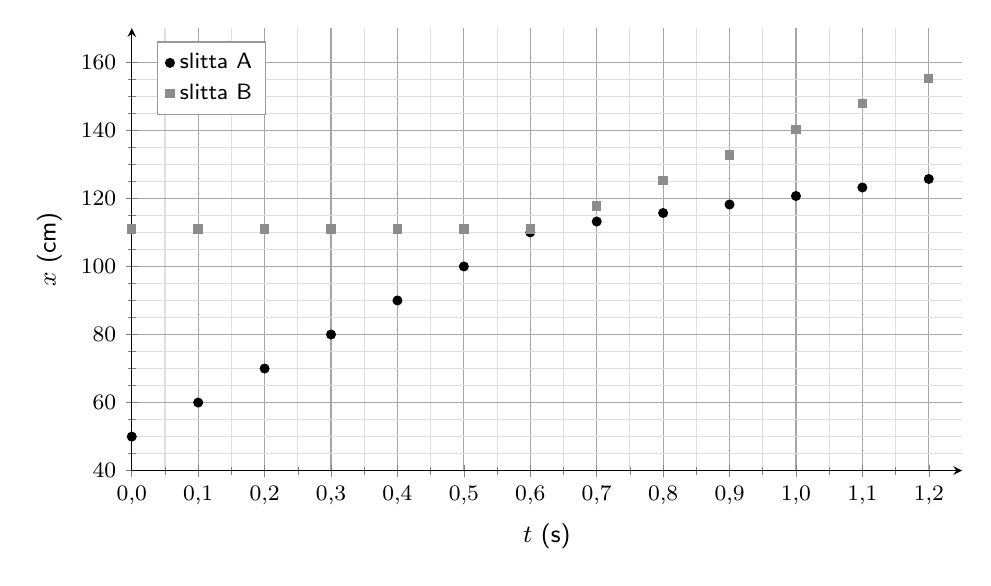
\begin{tikzpicture}
\begin{axis}[dati, width=\linewidth, height=7.2cm,
    xmin=0, xmax=1.25, ymin=40, ymax=170,
    xtick={0,0.1,...,1.2}, minor x tick num=1,
    ytick={40,60,...,160}, minor y tick num=3,
    xticklabel={\pgfmathprintnumber[fixed, fixed zerofill, precision=1, use comma]{\tick}},
    xlabel={$t$ (s)}, ylabel={$x$ (cm)}, legend pos=north west]
  \addplot[puntoA] coordinates {(0,50.0) (0.1,60.0) (0.2,70.0) (0.3,80.0) (0.4,90.0) (0.5,100.0)
    (0.6,110.0) (0.7,113.2) (0.8,115.7) (0.9,118.2) (1.0,120.7) (1.1,123.2) (1.2,125.7)};
  \addlegendentry{slitta A}
  \addplot[puntoB] coordinates {(0,111.0) (0.1,111.0) (0.2,111.0) (0.3,111.0) (0.4,111.0) (0.5,111.0)
    (0.6,111.0) (0.7,117.8) (0.8,125.3) (0.9,132.8) (1.0,140.3) (1.1,147.8) (1.2,155.3)};
  \addlegendentry{slitta B}
\end{axis}
\end{tikzpicture}
\end{center}

\begin{parts}
  \itemx Calcola la percentuale dell'energia cinetica iniziale che viene dissipata nell'urto.
  \itemx Le due slitte sono identiche. Ricava l'equazione oraria del centro di massa del sistema
    formato dalle due slitte, prima e dopo l'urto. Che cosa noti? Che legame c'è con la quantità di
    moto totale?
  \itemx Se al posto della gomma ci fosse stato un respingente di plastilina, che resta attaccato,
    come sarebbe cambiato il grafico $x$--$t$?
\end{parts}

\begin{solution}
Verso positivo verso destra. Dalle pendenze: prima $v_A = 1{,}00\unm{m/s}$, $v_B = 0$; dopo
(punti da $0{,}8$ a $1{,}2\unm{s}$) $v_A' = 10{,}0\unm{cm}/0{,}4\unm{s} = 0{,}25\unm{m/s}$ e
$v_B' = 30{,}0\unm{cm}/0{,}4\unm{s} = 0{,}75\unm{m/s}$.
Quantità di moto: $0{,}25\unm{kg\,m/s}$ prima e $0{,}0625 + 0{,}1875 = 0{,}25\unm{kg\,m/s}$
dopo.

\textbf{a.} Energia cinetica: $K_i = \tfrac12\,0{,}25\cdot 1{,}00^2 = 0{,}125\unm{J}$,
$K_f = \tfrac12\,0{,}25\,(0{,}25^2 + 0{,}75^2) = 0{,}078\unm{J}$. Dissipata:
$\dfrac{K_i - K_f}{K_i} = \dfrac{0{,}047}{0{,}125} = 37{,}5\%$ (gomma deformata e scaldata,
suono, vibrazioni). Urto anelastico: la velocità relativa passa da $1{,}00$ a $0{,}50\unm{m/s}$.

\textbf{b.} Le slitte sono identiche (lunghezza $L$): i centri stanno in $x_A - L/2$ e
$x_B + L/2$, quindi il centro di massa coincide con il punto medio dei due segni misurati,
$x_{CM} = (x_A + x_B)/2$. Dai dati: $80{,}5\unm{cm}$ a $t = 0$, $110{,}5\unm{cm}$ a $0{,}6\unm{s}$,
$140{,}5\unm{cm}$ a $1{,}2\unm{s}$, e i punti stanno sulla stessa retta anche durante l'urto:
\[ x_{CM}(t) = 0{,}805\unm{m} + (0{,}50\unm{m/s})\,t \]
prima e dopo l'urto. Il centro di massa si muove di moto rettilineo uniforme e non «si accorge»
dell'urto. La sua velocità è $v_{CM} = P/(m_A + m_B) = 0{,}25/0{,}50 = 0{,}50\unm{m/s}$: si
conserva perché si conserva la quantità di moto totale. Se gli studenti non hanno ancora visto il
centro di massa, basta la definizione $x_{CM} = (m_A x_A + m_B x_B)/(m_A + m_B)$ applicata ai centri.

\textbf{c.} Con la plastilina, dopo l'urto i due punti avanzano insieme a distanza costante:
un'unica retta (due rette parallele vicinissime) di pendenza $0{,}25/0{,}50 = 0{,}50\unm{m/s}$,
la stessa del centro di massa. L'energia cinetica finale sarebbe $0{,}0625\unm{J}$: se ne perde
metà ($50\%$).
\end{solution}

%% =========================================================================
\exercise[Slitte con magneti]
Sulla stessa rotaia, una slitta grande caricata con pesi ($500\unm{g}$ in tutto) viene lanciata a
$1{,}0\unm{m/s}$ contro una slitta piccola ($100\unm{g}$), ferma. Sulle due slitte sono montati
magneti che si respingono: le slitte non si toccano e l'urto è quasi elastico.
\medskip
\conqr{s=headon\&m1=0.5\&m2=0.1\&show=strobe\&tab=1\&g=x\&hide=bal,num\&lock=1}{%
\begin{parts}
  \itemx Senza fare calcoli, disegna il grafico $x$--$t$ che ti aspetti per le due slitte.
  \itemx Calcola la velocità del centro di massa, le velocità delle due slitte rispetto al centro
    di massa prima e dopo l'urto, e le velocità finali rispetto al laboratorio.
  \itemx Un compagno dice: «La slitta grande è cinque volte più pesante, quindi spinge la piccola
    molto più forte di quanto la piccola spinga lei». Ha ragione? Giustifica la risposta.
  \itemx Verifica con l'app (QR): confronta la foto stroboscopica con il grafico previsto e con le
    velocità calcolate, e correggi ciò che non torna.
\end{parts}}

\begin{solution}
\textbf{a.} Previsione attesa: la slitta grande rallenta ma prosegue, la piccola parte più veloce
di quanto andasse la grande. Nel grafico $x$--$t$ la retta della grande si piega verso una
pendenza minore, quella della piccola parte più ripida. Errori frequenti: la grande che si ferma
(come con masse uguali), la piccola più lenta della grande.

\textbf{b.} $v_{CM} = \dfrac{0{,}5\cdot 1{,}0}{0{,}6} = 0{,}83\unm{m/s}$. Rispetto al centro di
massa, prima: grande $1{,}0 - 0{,}83 = +0{,}17\unm{m/s}$, piccola $0 - 0{,}83 = -0{,}83\unm{m/s}$
(quantità di moto totale nulla: $0{,}5\cdot 0{,}17 - 0{,}1\cdot 0{,}83 = 0$). Nell'urto elastico le
velocità rispetto al centro di massa si invertono: dopo, grande $-0{,}17\unm{m/s}$, piccola
$+0{,}83\unm{m/s}$. Rispetto al laboratorio si somma $v_{CM}$: $v_g' = 0{,}83 - 0{,}17 =
0{,}67\unm{m/s}$, $v_p' = 0{,}83 + 0{,}83 = 1{,}67\unm{m/s}$. Stesso risultato delle formule
$v_g' = \frac{m_g - m_p}{m_g + m_p}\,v$ e $v_p' = \frac{2m_g}{m_g + m_p}\,v$.

\textbf{c.} No. Impulso sulla piccola: $0{,}1 \cdot 1{,}67 = +0{,}167\unm{N\,s}$; sulla grande:
$0{,}5\,(0{,}67 - 1{,}00) = -0{,}167\unm{N\,s}$. Per il terzo principio le forze sono uguali e
opposte e agiscono per lo stesso tempo, quindi gli impulsi sono uguali e opposti. Sono diverse
le variazioni di velocità, $\Delta v = J/m$: $-0{,}33\unm{m/s}$ per la grande, $+1{,}67\unm{m/s}$
per la piccola. È la misconcezione della dominanza: conviene far scrivere la risposta prima di
aprire la scena.

\textbf{d.} Il grafico dell'app deve mostrare la grande con pendenza $0{,}67\unm{m/s}$ e la
piccola con $1{,}67\unm{m/s}$; il pulsante \emph{Mostra} rivela bilancio e valori numerici.
\end{solution}

%% =========================================================================
\exercise[Carrelli con velcro e magneti]
Come per gli esperimenti effettuati in laboratorio, due sensori di posizione, ai due estremi della
rotaia, registrano il moto di due carrelli. Da un lato i carrelli hanno il velcro, dall'altro
magneti che si respingono. Il carrello A ha una massa aggiuntiva ($500\unm{g}$ in tutto), il
carrello B è scarico ($250\unm{g}$).
\medskip
\conqr{s=headon\&m1=0.5\&v1=0.5\&x2=1.4\&st=1\&show=strobe,mom\&tab=2}{%
\begin{parts}
  \itemx Con i lati a velcro affacciati: come vanno lanciati i due carrelli perché, dopo l'urto,
    restino fermi? Motiva la risposta.
  \itemx Ora i carrelli sono girati, con i magneti affacciati (urto quasi elastico). Si può fare in
    modo che dopo l'urto si fermi uno solo dei due? Trova almeno una soluzione e motivala.
  \itemx Verifica con l'app (QR) le risposte alle due domande precedenti; per la seconda togli il
    velcro.
\end{parts}}

\begin{solution}
\textbf{a.} I carrelli restano fermi se la quantità di moto totale è nulla:
$m_A v_A + m_B v_B = 0$, cioè $v_B = -2\,v_A$ (lanciati uno contro l'altro, B con velocità
doppia ma massa metà); per esempio $v_A = +0{,}25\unm{m/s}$ e $v_B = -0{,}50\unm{m/s}$. La
motivazione è la conservazione della quantità di moto: se prima le due quantità di moto sono
uguali e opposte (somma nulla) e i carrelli restano attaccati, dopo la somma è nulla solo se la
velocità comune è nulla. Con il diagramma a barre: prima due barre di uguale lunghezza e verso
opposto, dopo nessuna barra. L'energia cinetica
($0{,}016 + 0{,}031 = 0{,}047\unm{J}$ nell'esempio) sparisce tutta: è l'unico caso in cui un urto
la fa sparire tutta.

\textbf{b.} Con l'urto elastico si può fermare A. Le condizioni sono la conservazione della
quantità di moto e l'inversione della velocità relativa ($v_B' - v_A' = v_A - v_B$); con
$v_A' = 0$ si ottiene $v_B = -0{,}5\,v_A$. Per esempio $v_A = +0{,}60\unm{m/s}$,
$v_B = -0{,}30\unm{m/s}$: dopo l'urto A è fermo e B riparte a $+0{,}90\unm{m/s}$. Con B fermo
all'inizio non si riesce (servirebbero masse uguali). Fermare B è impossibile: B dovrebbe
allontanarsi da A più veloce di lui, e l'urto non avverrebbe.

\textbf{c.} Per la a basta la scena così com'è (velcro attivo) con $v_A$ e $v_B$ nel rapporto
trovato; per la b si toglie il velcro e si impostano le velocità. Sulla rotaia vera i magneti non
danno un urto perfettamente elastico e c'è un po' di attrito: A non si fermerebbe del tutto, e
questo è un buon punto di discussione, ma non è richiesto di provarlo.
\end{solution}

%% =========================================================================
\newpage
\exercise[Dischi sul tavolo a cuscino d'aria]
Su un tavolo a cuscino d'aria orizzontale, il disco A ($250\unm{g}$, diametro $9\unm{cm}$)
colpisce di striscio il disco B, identico e fermo. I bordi dei dischi sono rivestiti da un anello
elastico. Lo smartphone, fissato sopra il tavolo, riprende la scena; il grafico riporta le
posizioni dei centri ricavate con Tracker, ogni $0{,}1\unm{s}$, da $t = 0{,}4\unm{s}$ a
$t = 1{,}2\unm{s}$.

\begin{center}
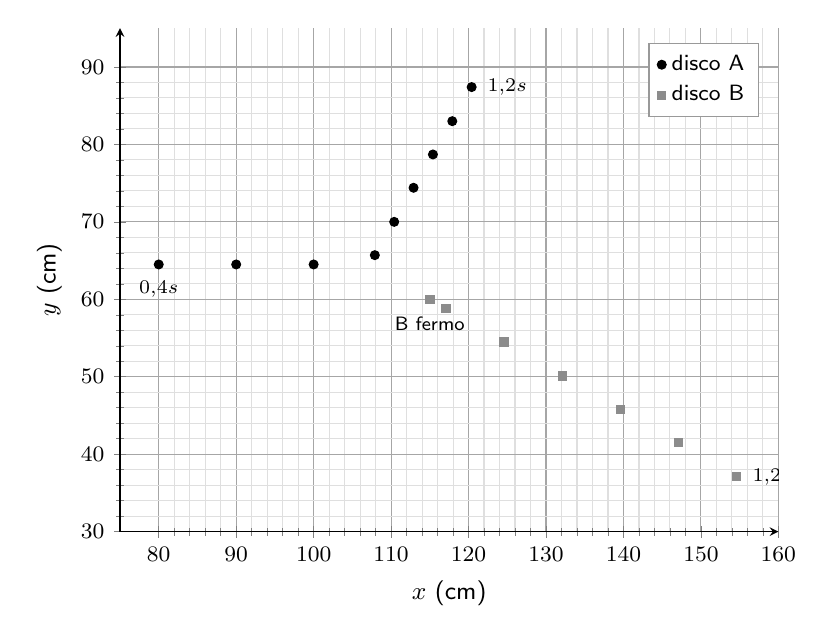
\begin{tikzpicture}
\begin{axis}[dati, axis equal image, width=.82\linewidth,
    xmin=75, xmax=160, ymin=30, ymax=95,
    xtick={80,90,...,160}, ytick={30,40,...,90}, minor tick num=4,
    xlabel={$x$ (cm)}, ylabel={$y$ (cm)}, legend pos=north east]
  \addplot[puntoA] coordinates {(80.0,64.5) (90.0,64.5) (100.0,64.5) (107.9,65.7) (110.4,70.0)
    (112.9,74.4) (115.4,78.7) (117.9,83.0) (120.4,87.4)};
  \addlegendentry{disco A}
  \addplot[puntoB] coordinates {(115.0,60.0) (117.1,58.8) (124.6,54.5) (132.1,50.1) (139.6,45.8)
    (147.1,41.5) (154.6,37.1)};
  \addlegendentry{disco B}
  \node[font=\scriptsize, anchor=north] at (axis cs:80,63.6) {$0{,}4\unm{s}$};
  \node[font=\scriptsize, anchor=west] at (axis cs:121.2,87.4) {$1{,}2\unm{s}$};
  \node[font=\scriptsize, anchor=north] at (axis cs:115,59) {B fermo};
  \node[font=\scriptsize, anchor=west] at (axis cs:155.4,37.1) {$1{,}2\unm{s}$};
\end{axis}
\end{tikzpicture}
\end{center}

\conqr{p=urti/s10\&tab=2}{%
\begin{parts}
  \itemx Dopo l'urto i due dischi partono ad angolo retto. È un caso? Verificalo con i dati, poi
    prova a spiegarlo partendo dalla quantità di moto, componente per componente, e dall'energia.
  \itemx Con l'app cambia il punto d'impatto e le masse: quando l'angolo smette di essere retto?
\end{parts}}

\begin{solution}
\textbf{a.} Prima: A a $1{,}00\unm{m/s}$ lungo $x$ ($10\unm{cm}$ ogni $0{,}1\unm{s}$). Dopo (punti
da $0{,}8$ a $1{,}2\unm{s}$): A $(0{,}25;\ 0{,}435)\unm{m/s}$, inclinata di $+60^\circ$;
B $(0{,}75;\ -0{,}435)\unm{m/s}$, inclinata di $-30^\circ$. L'angolo fra le traiettorie è
$90^\circ$. Componente $x$: $0{,}25 = 0{,}0625 + 0{,}1875\unm{kg\,m/s}$; componente $y$:
$0 = 0{,}109 - 0{,}109\unm{kg\,m/s}$. Energia: $0{,}125\unm{J}$ prima,
$0{,}031 + 0{,}094 = 0{,}125\unm{J}$ dopo, quindi l'urto è elastico.
Spiegazione: con masse uguali $\vec p_A = \vec p_A\,' + \vec p_B\,'$ è un triangolo di vettori;
la conservazione dell'energia, divisa per $m/2$, dà $p_A^2 = p_A'^2 + p_B'^2$. Per l'inverso del
teorema di Pitagora il triangolo è rettangolo.

\textbf{b.} L'angolo resta retto per ogni punto d'impatto (tranne l'urto frontale) solo con masse
uguali e urto elastico. Se A è più pesante l'angolo è minore di $90^\circ$, se è più leggero è
maggiore; con un urto anelastico è minore. Spunto facoltativo, non nel testo: nelle fotografie in camera a nebbia una particella $\alpha$ su
un nucleo di elio (masse uguali) lascia una traccia a «Y» ad angolo retto, segno di urto elastico. Le fotografie sono nella Nobel
Lecture di P.\,M.\,S. Blackett (1948), figure 1--3, con urti su ossigeno, idrogeno ed elio:
\url{https://nobelprize.org/uploads/2018/06/blackett-lecture.pdf}.
\end{solution}

\end{document}
"
\usepackage[subject=physics, seed=2026]{fancytests}
\usepackage{lmodern}
\renewcommand*\familydefault{\sfdefault}
\usepackage[T1]{fontenc}
\usepackage{qrcode}
\usepackage{url}

\geometry{a4paper, top=15mm, bottom=15mm, left=17.5mm, right=17.5mm}
\pagestyle{empty}
\linespread{1.12}

\testsetup{labels=boxed, mcq=none, autoclose=false, scores=false}

%% ---------------------------------------------------------------------------
%% QR verso una scena di Collision Lab: testo a sinistra, QR a destra
%% \conqr{frammento dopo #, con \& al posto di &}{testo}
%% ---------------------------------------------------------------------------
\newcommand{\appurl}{https://labs.matephis.com/collision-lab/}
\newcommand{\conqr}[2]{%
  \par\smallskip\noindent
  \begin{minipage}[c]{\dimexpr\linewidth-3.1cm}#2\end{minipage}\hfill
  \begin{minipage}[c]{2.6cm}\centering
    \qrcode[height=2.4cm]{\appurl\##1}\par
    {\scriptsize\color{black!55}Collision Lab}
  \end{minipage}\par\smallskip}

%% grafici di dati: assi a sinistra, griglia fitta, punti senza linee
\pgfplotsset{
  dati/.style={
    axis lines=left, grid=both, grid style={gray!70}, minor grid style={gray!25},
    tick label style={font=\footnotesize}, label style={font=\small},
    legend style={font=\footnotesize, draw=black!40, fill=white},
    legend cell align=left,
  },
  puntoA/.style={only marks, mark=*, mark size=1.6pt, black},
  puntoB/.style={only marks, mark=square*, mark size=1.5pt, black!45},
}

\begin{document}

\noindent{\Large\bfseries Fisica \textperiodcentered{} Urti in laboratorio}\par
\vspace{.4em}\noindent{\color{black!45}\rule{\textwidth}{.4pt}}\par\vspace{.4em}

\noindent Dove c'è un QR, la scena si apre in una web app. Le foto stroboscopiche sono scattate a intervalli di $0{,}1\unm{s}$.\par

\begin{solution}[Indicazioni per il docente]
\textbf{Obiettivo.} Quattro urti che coprono i casi principali: anelastico con dissipazione di
energia e moto del centro di massa (es.~1), elastico tra masse diverse nel riferimento del centro
di massa, con impulso e terzo principio (es.~2), completamente anelastico con quantità di moto
totale nulla ed elastico con un corpo che si ferma (es.~3), elastico in due dimensioni (es.~4).
Restano fuori le esplosioni.

\textbf{Struttura.} Ogni esercizio cambia punto di partenza e di arrivo, perché gli studenti non
applichino una procedura fissa: dati $\to$ energia dissipata e centro di massa (1); descrizione
$\to$ grafico previsto, calcolo, verifica (2); obiettivo $\to$ progetto della scena, verifica (3);
osservazione $\to$ spiegazione (4). Negli esercizi 2 e 3 l'app serve solo alla fine, per
controllare le risposte già date. Le domande sono aperte; conviene pretendere che ogni risposta
sia giustificata con almeno una rappresentazione.

\textbf{Tempi.} Circa un'ora: 10--15 minuti per esercizio, di più per il 3 e il 4. In
alternativa, i gruppi svolgono esercizi diversi e poi li presentano.

\textbf{Dati.} I grafici degli esercizi 1 e 4 sono stati generati con Collision Lab (stesse
masse e velocità), arrotondati al millimetro, senza rumore. Nei fotogrammi in cui i corpi sono a
contatto (es.~1, $t = 0{,}6$--$0{,}7\unm{s}$) i punti non stanno sulle rette: le velocità vanno
ricavate da punti lontani dall'urto. Nell'es.~1, $x_A$ e $x_B$ sono le estremità che si toccano,
quindi all'urto $x_A \approx x_B$.

\textbf{QR.} Es.~2: scena bloccata, aperta sul grafico $x$--$t$, con bilancio e valori numerici
nascosti; dopo previsione e calcoli, il pulsante \emph{Mostra} li rivela. Es.~3: si apre sulla
scheda \emph{Imposta}, con il velcro attivo e i vettori della quantità di moto; per verificare la
domanda b si toglie il velcro. Es.~4: preset \texttt{urti/s10}, sulla scheda \emph{Imposta}, per
cambiare masse e parametro d'urto. Nell'app il corpo A sta sempre a sinistra.
\end{solution}

%% =========================================================================
\exercise[Slitte con respingente di gomma]
Su una rotaia a cuscino d'aria orizzontale, la slitta A ($250\unm{g}$) viene spinta contro la
slitta B ($250\unm{g}$), ferma. Sul muso di A è montato un respingente ad anello di gomma. Il
grafico riporta le posizioni ricavate dal video con Tracker, ogni $0{,}1\unm{s}$: $x_A$ è la
posizione del respingente di A, $x_B$ quella del retro di B.

\begin{center}
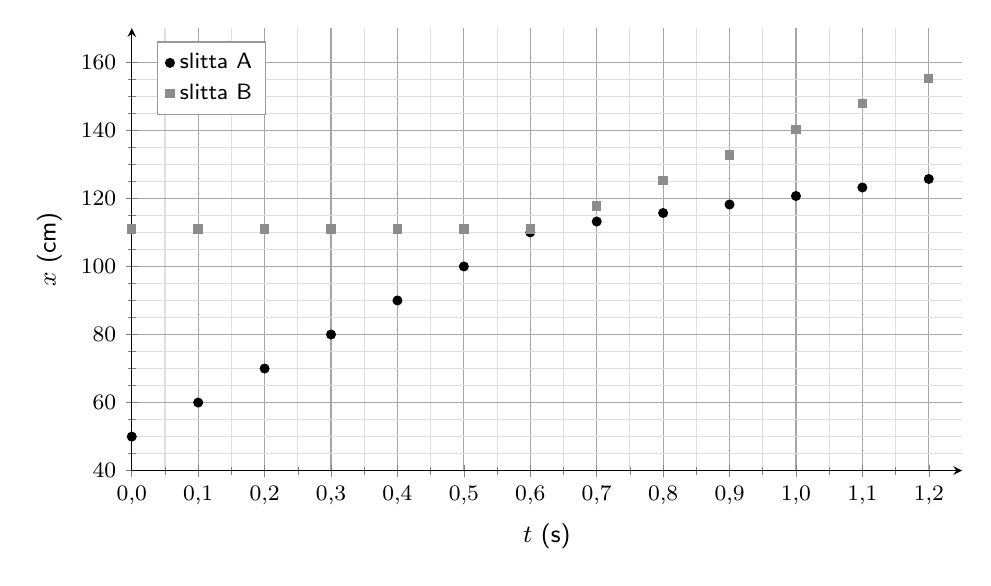
\begin{tikzpicture}
\begin{axis}[dati, width=\linewidth, height=7.2cm,
    xmin=0, xmax=1.25, ymin=40, ymax=170,
    xtick={0,0.1,...,1.2}, minor x tick num=1,
    ytick={40,60,...,160}, minor y tick num=3,
    xticklabel={\pgfmathprintnumber[fixed, fixed zerofill, precision=1, use comma]{\tick}},
    xlabel={$t$ (s)}, ylabel={$x$ (cm)}, legend pos=north west]
  \addplot[puntoA] coordinates {(0,50.0) (0.1,60.0) (0.2,70.0) (0.3,80.0) (0.4,90.0) (0.5,100.0)
    (0.6,110.0) (0.7,113.2) (0.8,115.7) (0.9,118.2) (1.0,120.7) (1.1,123.2) (1.2,125.7)};
  \addlegendentry{slitta A}
  \addplot[puntoB] coordinates {(0,111.0) (0.1,111.0) (0.2,111.0) (0.3,111.0) (0.4,111.0) (0.5,111.0)
    (0.6,111.0) (0.7,117.8) (0.8,125.3) (0.9,132.8) (1.0,140.3) (1.1,147.8) (1.2,155.3)};
  \addlegendentry{slitta B}
\end{axis}
\end{tikzpicture}
\end{center}

\begin{parts}
  \itemx Calcola la percentuale dell'energia cinetica iniziale che viene dissipata nell'urto.
  \itemx Le due slitte sono identiche. Ricava l'equazione oraria del centro di massa del sistema
    formato dalle due slitte, prima e dopo l'urto. Che cosa noti? Che legame c'è con la quantità di
    moto totale?
  \itemx Se al posto della gomma ci fosse stato un respingente di plastilina, che resta attaccato,
    come sarebbe cambiato il grafico $x$--$t$?
\end{parts}

\begin{solution}
Verso positivo verso destra. Dalle pendenze: prima $v_A = 1{,}00\unm{m/s}$, $v_B = 0$; dopo
(punti da $0{,}8$ a $1{,}2\unm{s}$) $v_A' = 10{,}0\unm{cm}/0{,}4\unm{s} = 0{,}25\unm{m/s}$ e
$v_B' = 30{,}0\unm{cm}/0{,}4\unm{s} = 0{,}75\unm{m/s}$.
Quantità di moto: $0{,}25\unm{kg\,m/s}$ prima e $0{,}0625 + 0{,}1875 = 0{,}25\unm{kg\,m/s}$
dopo.

\textbf{a.} Energia cinetica: $K_i = \tfrac12\,0{,}25\cdot 1{,}00^2 = 0{,}125\unm{J}$,
$K_f = \tfrac12\,0{,}25\,(0{,}25^2 + 0{,}75^2) = 0{,}078\unm{J}$. Dissipata:
$\dfrac{K_i - K_f}{K_i} = \dfrac{0{,}047}{0{,}125} = 37{,}5\%$ (gomma deformata e scaldata,
suono, vibrazioni). Urto anelastico: la velocità relativa passa da $1{,}00$ a $0{,}50\unm{m/s}$.

\textbf{b.} Le slitte sono identiche (lunghezza $L$): i centri stanno in $x_A - L/2$ e
$x_B + L/2$, quindi il centro di massa coincide con il punto medio dei due segni misurati,
$x_{CM} = (x_A + x_B)/2$. Dai dati: $80{,}5\unm{cm}$ a $t = 0$, $110{,}5\unm{cm}$ a $0{,}6\unm{s}$,
$140{,}5\unm{cm}$ a $1{,}2\unm{s}$, e i punti stanno sulla stessa retta anche durante l'urto:
\[ x_{CM}(t) = 0{,}805\unm{m} + (0{,}50\unm{m/s})\,t \]
prima e dopo l'urto. Il centro di massa si muove di moto rettilineo uniforme e non «si accorge»
dell'urto. La sua velocità è $v_{CM} = P/(m_A + m_B) = 0{,}25/0{,}50 = 0{,}50\unm{m/s}$: si
conserva perché si conserva la quantità di moto totale. Se gli studenti non hanno ancora visto il
centro di massa, basta la definizione $x_{CM} = (m_A x_A + m_B x_B)/(m_A + m_B)$ applicata ai centri.

\textbf{c.} Con la plastilina, dopo l'urto i due punti avanzano insieme a distanza costante:
un'unica retta (due rette parallele vicinissime) di pendenza $0{,}25/0{,}50 = 0{,}50\unm{m/s}$,
la stessa del centro di massa. L'energia cinetica finale sarebbe $0{,}0625\unm{J}$: se ne perde
metà ($50\%$).
\end{solution}

%% =========================================================================
\exercise[Slitte con magneti]
Sulla stessa rotaia, una slitta grande caricata con pesi ($500\unm{g}$ in tutto) viene lanciata a
$1{,}0\unm{m/s}$ contro una slitta piccola ($100\unm{g}$), ferma. Sulle due slitte sono montati
magneti che si respingono: le slitte non si toccano e l'urto è quasi elastico.
\medskip
\conqr{s=headon\&m1=0.5\&m2=0.1\&show=strobe\&tab=1\&g=x\&hide=bal,num\&lock=1}{%
\begin{parts}
  \itemx Senza fare calcoli, disegna il grafico $x$--$t$ che ti aspetti per le due slitte.
  \itemx Calcola la velocità del centro di massa, le velocità delle due slitte rispetto al centro
    di massa prima e dopo l'urto, e le velocità finali rispetto al laboratorio.
  \itemx Un compagno dice: «La slitta grande è cinque volte più pesante, quindi spinge la piccola
    molto più forte di quanto la piccola spinga lei». Ha ragione? Giustifica la risposta.
  \itemx Verifica con l'app (QR): confronta la foto stroboscopica con il grafico previsto e con le
    velocità calcolate, e correggi ciò che non torna.
\end{parts}}

\begin{solution}
\textbf{a.} Previsione attesa: la slitta grande rallenta ma prosegue, la piccola parte più veloce
di quanto andasse la grande. Nel grafico $x$--$t$ la retta della grande si piega verso una
pendenza minore, quella della piccola parte più ripida. Errori frequenti: la grande che si ferma
(come con masse uguali), la piccola più lenta della grande.

\textbf{b.} $v_{CM} = \dfrac{0{,}5\cdot 1{,}0}{0{,}6} = 0{,}83\unm{m/s}$. Rispetto al centro di
massa, prima: grande $1{,}0 - 0{,}83 = +0{,}17\unm{m/s}$, piccola $0 - 0{,}83 = -0{,}83\unm{m/s}$
(quantità di moto totale nulla: $0{,}5\cdot 0{,}17 - 0{,}1\cdot 0{,}83 = 0$). Nell'urto elastico le
velocità rispetto al centro di massa si invertono: dopo, grande $-0{,}17\unm{m/s}$, piccola
$+0{,}83\unm{m/s}$. Rispetto al laboratorio si somma $v_{CM}$: $v_g' = 0{,}83 - 0{,}17 =
0{,}67\unm{m/s}$, $v_p' = 0{,}83 + 0{,}83 = 1{,}67\unm{m/s}$. Stesso risultato delle formule
$v_g' = \frac{m_g - m_p}{m_g + m_p}\,v$ e $v_p' = \frac{2m_g}{m_g + m_p}\,v$.

\textbf{c.} No. Impulso sulla piccola: $0{,}1 \cdot 1{,}67 = +0{,}167\unm{N\,s}$; sulla grande:
$0{,}5\,(0{,}67 - 1{,}00) = -0{,}167\unm{N\,s}$. Per il terzo principio le forze sono uguali e
opposte e agiscono per lo stesso tempo, quindi gli impulsi sono uguali e opposti. Sono diverse
le variazioni di velocità, $\Delta v = J/m$: $-0{,}33\unm{m/s}$ per la grande, $+1{,}67\unm{m/s}$
per la piccola. È la misconcezione della dominanza: conviene far scrivere la risposta prima di
aprire la scena.

\textbf{d.} Il grafico dell'app deve mostrare la grande con pendenza $0{,}67\unm{m/s}$ e la
piccola con $1{,}67\unm{m/s}$; il pulsante \emph{Mostra} rivela bilancio e valori numerici.
\end{solution}

%% =========================================================================
\exercise[Carrelli con velcro e magneti]
Come per gli esperimenti effettuati in laboratorio, due sensori di posizione, ai due estremi della
rotaia, registrano il moto di due carrelli. Da un lato i carrelli hanno il velcro, dall'altro
magneti che si respingono. Il carrello A ha una massa aggiuntiva ($500\unm{g}$ in tutto), il
carrello B è scarico ($250\unm{g}$).
\medskip
\conqr{s=headon\&m1=0.5\&v1=0.5\&x2=1.4\&st=1\&show=strobe,mom\&tab=2}{%
\begin{parts}
  \itemx Con i lati a velcro affacciati: come vanno lanciati i due carrelli perché, dopo l'urto,
    restino fermi? Motiva la risposta.
  \itemx Ora i carrelli sono girati, con i magneti affacciati (urto quasi elastico). Si può fare in
    modo che dopo l'urto si fermi uno solo dei due? Trova almeno una soluzione e motivala.
  \itemx Verifica con l'app (QR) le risposte alle due domande precedenti; per la seconda togli il
    velcro.
\end{parts}}

\begin{solution}
\textbf{a.} I carrelli restano fermi se la quantità di moto totale è nulla:
$m_A v_A + m_B v_B = 0$, cioè $v_B = -2\,v_A$ (lanciati uno contro l'altro, B con velocità
doppia ma massa metà); per esempio $v_A = +0{,}25\unm{m/s}$ e $v_B = -0{,}50\unm{m/s}$. La
motivazione è la conservazione della quantità di moto: se prima le due quantità di moto sono
uguali e opposte (somma nulla) e i carrelli restano attaccati, dopo la somma è nulla solo se la
velocità comune è nulla. Con il diagramma a barre: prima due barre di uguale lunghezza e verso
opposto, dopo nessuna barra. L'energia cinetica
($0{,}016 + 0{,}031 = 0{,}047\unm{J}$ nell'esempio) sparisce tutta: è l'unico caso in cui un urto
la fa sparire tutta.

\textbf{b.} Con l'urto elastico si può fermare A. Le condizioni sono la conservazione della
quantità di moto e l'inversione della velocità relativa ($v_B' - v_A' = v_A - v_B$); con
$v_A' = 0$ si ottiene $v_B = -0{,}5\,v_A$. Per esempio $v_A = +0{,}60\unm{m/s}$,
$v_B = -0{,}30\unm{m/s}$: dopo l'urto A è fermo e B riparte a $+0{,}90\unm{m/s}$. Con B fermo
all'inizio non si riesce (servirebbero masse uguali). Fermare B è impossibile: B dovrebbe
allontanarsi da A più veloce di lui, e l'urto non avverrebbe.

\textbf{c.} Per la a basta la scena così com'è (velcro attivo) con $v_A$ e $v_B$ nel rapporto
trovato; per la b si toglie il velcro e si impostano le velocità. Sulla rotaia vera i magneti non
danno un urto perfettamente elastico e c'è un po' di attrito: A non si fermerebbe del tutto, e
questo è un buon punto di discussione, ma non è richiesto di provarlo.
\end{solution}

%% =========================================================================
\newpage
\exercise[Dischi sul tavolo a cuscino d'aria]
Su un tavolo a cuscino d'aria orizzontale, il disco A ($250\unm{g}$, diametro $9\unm{cm}$)
colpisce di striscio il disco B, identico e fermo. I bordi dei dischi sono rivestiti da un anello
elastico. Lo smartphone, fissato sopra il tavolo, riprende la scena; il grafico riporta le
posizioni dei centri ricavate con Tracker, ogni $0{,}1\unm{s}$, da $t = 0{,}4\unm{s}$ a
$t = 1{,}2\unm{s}$.

\begin{center}
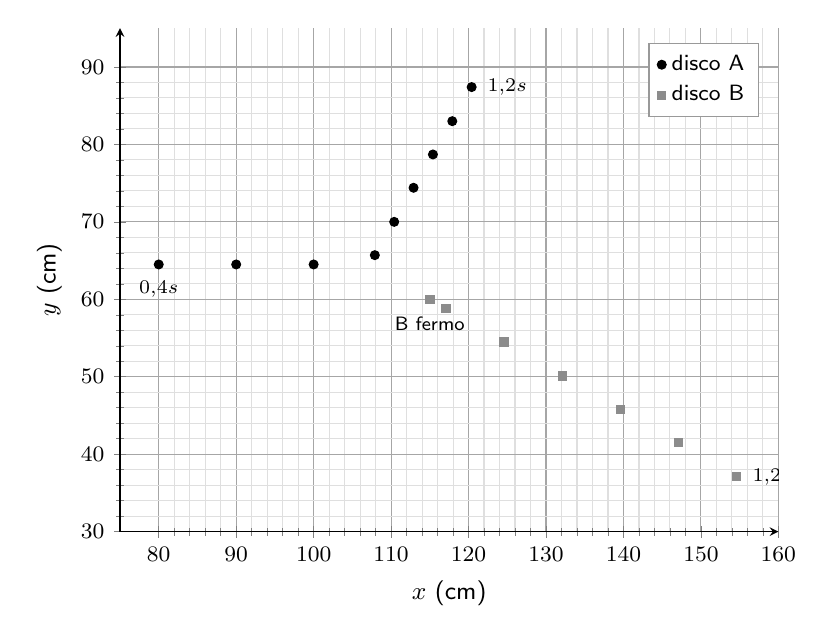
\begin{tikzpicture}
\begin{axis}[dati, axis equal image, width=.82\linewidth,
    xmin=75, xmax=160, ymin=30, ymax=95,
    xtick={80,90,...,160}, ytick={30,40,...,90}, minor tick num=4,
    xlabel={$x$ (cm)}, ylabel={$y$ (cm)}, legend pos=north east]
  \addplot[puntoA] coordinates {(80.0,64.5) (90.0,64.5) (100.0,64.5) (107.9,65.7) (110.4,70.0)
    (112.9,74.4) (115.4,78.7) (117.9,83.0) (120.4,87.4)};
  \addlegendentry{disco A}
  \addplot[puntoB] coordinates {(115.0,60.0) (117.1,58.8) (124.6,54.5) (132.1,50.1) (139.6,45.8)
    (147.1,41.5) (154.6,37.1)};
  \addlegendentry{disco B}
  \node[font=\scriptsize, anchor=north] at (axis cs:80,63.6) {$0{,}4\unm{s}$};
  \node[font=\scriptsize, anchor=west] at (axis cs:121.2,87.4) {$1{,}2\unm{s}$};
  \node[font=\scriptsize, anchor=north] at (axis cs:115,59) {B fermo};
  \node[font=\scriptsize, anchor=west] at (axis cs:155.4,37.1) {$1{,}2\unm{s}$};
\end{axis}
\end{tikzpicture}
\end{center}

\conqr{p=urti/s10\&tab=2}{%
\begin{parts}
  \itemx Dopo l'urto i due dischi partono ad angolo retto. È un caso? Verificalo con i dati, poi
    prova a spiegarlo partendo dalla quantità di moto, componente per componente, e dall'energia.
  \itemx Con l'app cambia il punto d'impatto e le masse: quando l'angolo smette di essere retto?
\end{parts}}

\begin{solution}
\textbf{a.} Prima: A a $1{,}00\unm{m/s}$ lungo $x$ ($10\unm{cm}$ ogni $0{,}1\unm{s}$). Dopo (punti
da $0{,}8$ a $1{,}2\unm{s}$): A $(0{,}25;\ 0{,}435)\unm{m/s}$, inclinata di $+60^\circ$;
B $(0{,}75;\ -0{,}435)\unm{m/s}$, inclinata di $-30^\circ$. L'angolo fra le traiettorie è
$90^\circ$. Componente $x$: $0{,}25 = 0{,}0625 + 0{,}1875\unm{kg\,m/s}$; componente $y$:
$0 = 0{,}109 - 0{,}109\unm{kg\,m/s}$. Energia: $0{,}125\unm{J}$ prima,
$0{,}031 + 0{,}094 = 0{,}125\unm{J}$ dopo, quindi l'urto è elastico.
Spiegazione: con masse uguali $\vec p_A = \vec p_A\,' + \vec p_B\,'$ è un triangolo di vettori;
la conservazione dell'energia, divisa per $m/2$, dà $p_A^2 = p_A'^2 + p_B'^2$. Per l'inverso del
teorema di Pitagora il triangolo è rettangolo.

\textbf{b.} L'angolo resta retto per ogni punto d'impatto (tranne l'urto frontale) solo con masse
uguali e urto elastico. Se A è più pesante l'angolo è minore di $90^\circ$, se è più leggero è
maggiore; con un urto anelastico è minore. Spunto facoltativo, non nel testo: nelle fotografie in camera a nebbia una particella $\alpha$ su
un nucleo di elio (masse uguali) lascia una traccia a «Y» ad angolo retto, segno di urto elastico. Le fotografie sono nella Nobel
Lecture di P.\,M.\,S. Blackett (1948), figure 1--3, con urti su ossigeno, idrogeno ed elio:
\url{https://nobelprize.org/uploads/2018/06/blackett-lecture.pdf}.
\end{solution}

\end{document}
"
\usepackage[subject=physics, seed=2026]{fancytests}
\usepackage{lmodern}
\renewcommand*\familydefault{\sfdefault}
\usepackage[T1]{fontenc}
\usepackage{qrcode}
\usepackage{url}

\geometry{a4paper, top=15mm, bottom=15mm, left=17.5mm, right=17.5mm}
\pagestyle{empty}
\linespread{1.12}

\testsetup{labels=boxed, mcq=none, autoclose=false, scores=false}

%% ---------------------------------------------------------------------------
%% QR verso una scena di Collision Lab: testo a sinistra, QR a destra
%% \conqr{frammento dopo #, con \& al posto di &}{testo}
%% ---------------------------------------------------------------------------
\newcommand{\appurl}{https://labs.matephis.com/collision-lab/}
\newcommand{\conqr}[2]{%
  \par\smallskip\noindent
  \begin{minipage}[c]{\dimexpr\linewidth-3.1cm}#2\end{minipage}\hfill
  \begin{minipage}[c]{2.6cm}\centering
    \qrcode[height=2.4cm]{\appurl\##1}\par
    {\scriptsize\color{black!55}Collision Lab}
  \end{minipage}\par\smallskip}

%% grafici di dati: assi a sinistra, griglia fitta, punti senza linee
\pgfplotsset{
  dati/.style={
    axis lines=left, grid=both, grid style={gray!70}, minor grid style={gray!25},
    tick label style={font=\footnotesize}, label style={font=\small},
    legend style={font=\footnotesize, draw=black!40, fill=white},
    legend cell align=left,
  },
  puntoA/.style={only marks, mark=*, mark size=1.6pt, black},
  puntoB/.style={only marks, mark=square*, mark size=1.5pt, black!45},
}

\begin{document}

\noindent{\Large\bfseries Fisica \textperiodcentered{} Urti in laboratorio}\par
\vspace{.4em}\noindent{\color{black!45}\rule{\textwidth}{.4pt}}\par\vspace{.4em}

\noindent Dove c'è un QR, la scena si apre in una web app. Le foto stroboscopiche sono scattate a intervalli di $0{,}1\unm{s}$.\par

\begin{solution}[Indicazioni per il docente]
\textbf{Obiettivo.} Quattro urti che coprono i casi principali: anelastico con dissipazione di
energia e moto del centro di massa (es.~1), elastico tra masse diverse nel riferimento del centro
di massa, con impulso e terzo principio (es.~2), completamente anelastico con quantità di moto
totale nulla ed elastico con un corpo che si ferma (es.~3), elastico in due dimensioni (es.~4).
Restano fuori le esplosioni.

\textbf{Struttura.} Ogni esercizio cambia punto di partenza e di arrivo, perché gli studenti non
applichino una procedura fissa: dati $\to$ energia dissipata e centro di massa (1); descrizione
$\to$ grafico previsto, calcolo, verifica (2); obiettivo $\to$ progetto della scena, verifica (3);
osservazione $\to$ spiegazione (4). Negli esercizi 2 e 3 l'app serve solo alla fine, per
controllare le risposte già date. Le domande sono aperte; conviene pretendere che ogni risposta
sia giustificata con almeno una rappresentazione.

\textbf{Tempi.} Circa un'ora: 10--15 minuti per esercizio, di più per il 3 e il 4. In
alternativa, i gruppi svolgono esercizi diversi e poi li presentano.

\textbf{Dati.} I grafici degli esercizi 1 e 4 sono stati generati con Collision Lab (stesse
masse e velocità), arrotondati al millimetro, senza rumore. Nei fotogrammi in cui i corpi sono a
contatto (es.~1, $t = 0{,}6$--$0{,}7\unm{s}$) i punti non stanno sulle rette: le velocità vanno
ricavate da punti lontani dall'urto. Nell'es.~1, $x_A$ e $x_B$ sono le estremità che si toccano,
quindi all'urto $x_A \approx x_B$.

\textbf{QR.} Es.~2: scena bloccata, aperta sul grafico $x$--$t$, con bilancio e valori numerici
nascosti; dopo previsione e calcoli, il pulsante \emph{Mostra} li rivela. Es.~3: si apre sulla
scheda \emph{Imposta}, con il velcro attivo e i vettori della quantità di moto; per verificare la
domanda b si toglie il velcro. Es.~4: preset \texttt{urti/s10}, sulla scheda \emph{Imposta}, per
cambiare masse e parametro d'urto. Nell'app il corpo A sta sempre a sinistra.
\end{solution}

%% =========================================================================
\exercise[Slitte con respingente di gomma]
Su una rotaia a cuscino d'aria orizzontale, la slitta A ($250\unm{g}$) viene spinta contro la
slitta B ($250\unm{g}$), ferma. Sul muso di A è montato un respingente ad anello di gomma. Il
grafico riporta le posizioni ricavate dal video con Tracker, ogni $0{,}1\unm{s}$: $x_A$ è la
posizione del respingente di A, $x_B$ quella del retro di B.

\begin{center}
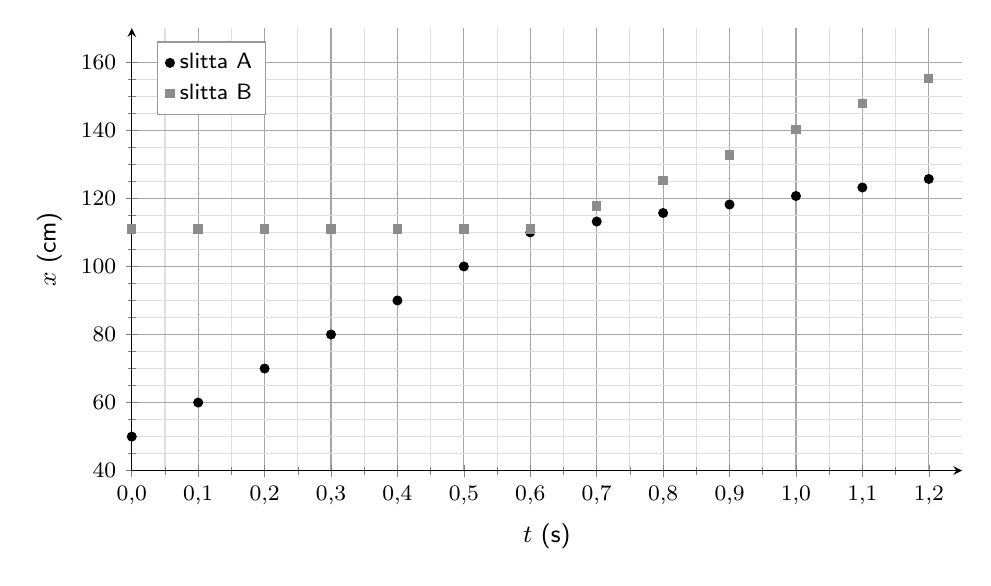
\begin{tikzpicture}
\begin{axis}[dati, width=\linewidth, height=7.2cm,
    xmin=0, xmax=1.25, ymin=40, ymax=170,
    xtick={0,0.1,...,1.2}, minor x tick num=1,
    ytick={40,60,...,160}, minor y tick num=3,
    xticklabel={\pgfmathprintnumber[fixed, fixed zerofill, precision=1, use comma]{\tick}},
    xlabel={$t$ (s)}, ylabel={$x$ (cm)}, legend pos=north west]
  \addplot[puntoA] coordinates {(0,50.0) (0.1,60.0) (0.2,70.0) (0.3,80.0) (0.4,90.0) (0.5,100.0)
    (0.6,110.0) (0.7,113.2) (0.8,115.7) (0.9,118.2) (1.0,120.7) (1.1,123.2) (1.2,125.7)};
  \addlegendentry{slitta A}
  \addplot[puntoB] coordinates {(0,111.0) (0.1,111.0) (0.2,111.0) (0.3,111.0) (0.4,111.0) (0.5,111.0)
    (0.6,111.0) (0.7,117.8) (0.8,125.3) (0.9,132.8) (1.0,140.3) (1.1,147.8) (1.2,155.3)};
  \addlegendentry{slitta B}
\end{axis}
\end{tikzpicture}
\end{center}

\begin{parts}
  \itemx Calcola la percentuale dell'energia cinetica iniziale che viene dissipata nell'urto.
  \itemx Le due slitte sono identiche. Ricava l'equazione oraria del centro di massa del sistema
    formato dalle due slitte, prima e dopo l'urto. Che cosa noti? Che legame c'è con la quantità di
    moto totale?
  \itemx Se al posto della gomma ci fosse stato un respingente di plastilina, che resta attaccato,
    come sarebbe cambiato il grafico $x$--$t$?
\end{parts}

\begin{solution}
Verso positivo verso destra. Dalle pendenze: prima $v_A = 1{,}00\unm{m/s}$, $v_B = 0$; dopo
(punti da $0{,}8$ a $1{,}2\unm{s}$) $v_A' = 10{,}0\unm{cm}/0{,}4\unm{s} = 0{,}25\unm{m/s}$ e
$v_B' = 30{,}0\unm{cm}/0{,}4\unm{s} = 0{,}75\unm{m/s}$.
Quantità di moto: $0{,}25\unm{kg\,m/s}$ prima e $0{,}0625 + 0{,}1875 = 0{,}25\unm{kg\,m/s}$
dopo.

\textbf{a.} Energia cinetica: $K_i = \tfrac12\,0{,}25\cdot 1{,}00^2 = 0{,}125\unm{J}$,
$K_f = \tfrac12\,0{,}25\,(0{,}25^2 + 0{,}75^2) = 0{,}078\unm{J}$. Dissipata:
$\dfrac{K_i - K_f}{K_i} = \dfrac{0{,}047}{0{,}125} = 37{,}5\%$ (gomma deformata e scaldata,
suono, vibrazioni). Urto anelastico: la velocità relativa passa da $1{,}00$ a $0{,}50\unm{m/s}$.

\textbf{b.} Le slitte sono identiche (lunghezza $L$): i centri stanno in $x_A - L/2$ e
$x_B + L/2$, quindi il centro di massa coincide con il punto medio dei due segni misurati,
$x_{CM} = (x_A + x_B)/2$. Dai dati: $80{,}5\unm{cm}$ a $t = 0$, $110{,}5\unm{cm}$ a $0{,}6\unm{s}$,
$140{,}5\unm{cm}$ a $1{,}2\unm{s}$, e i punti stanno sulla stessa retta anche durante l'urto:
\[ x_{CM}(t) = 0{,}805\unm{m} + (0{,}50\unm{m/s})\,t \]
prima e dopo l'urto. Il centro di massa si muove di moto rettilineo uniforme e non «si accorge»
dell'urto. La sua velocità è $v_{CM} = P/(m_A + m_B) = 0{,}25/0{,}50 = 0{,}50\unm{m/s}$: si
conserva perché si conserva la quantità di moto totale. Se gli studenti non hanno ancora visto il
centro di massa, basta la definizione $x_{CM} = (m_A x_A + m_B x_B)/(m_A + m_B)$ applicata ai centri.

\textbf{c.} Con la plastilina, dopo l'urto i due punti avanzano insieme a distanza costante:
un'unica retta (due rette parallele vicinissime) di pendenza $0{,}25/0{,}50 = 0{,}50\unm{m/s}$,
la stessa del centro di massa. L'energia cinetica finale sarebbe $0{,}0625\unm{J}$: se ne perde
metà ($50\%$).
\end{solution}

%% =========================================================================
\exercise[Slitte con magneti]
Sulla stessa rotaia, una slitta grande caricata con pesi ($500\unm{g}$ in tutto) viene lanciata a
$1{,}0\unm{m/s}$ contro una slitta piccola ($100\unm{g}$), ferma. Sulle due slitte sono montati
magneti che si respingono: le slitte non si toccano e l'urto è quasi elastico.
\medskip
\conqr{s=headon\&m1=0.5\&m2=0.1\&show=strobe\&tab=1\&g=x\&hide=bal,num\&lock=1}{%
\begin{parts}
  \itemx Senza fare calcoli, disegna il grafico $x$--$t$ che ti aspetti per le due slitte.
  \itemx Calcola la velocità del centro di massa, le velocità delle due slitte rispetto al centro
    di massa prima e dopo l'urto, e le velocità finali rispetto al laboratorio.
  \itemx Un compagno dice: «La slitta grande è cinque volte più pesante, quindi spinge la piccola
    molto più forte di quanto la piccola spinga lei». Ha ragione? Giustifica la risposta.
  \itemx Verifica con l'app (QR): confronta la foto stroboscopica con il grafico previsto e con le
    velocità calcolate, e correggi ciò che non torna.
\end{parts}}

\begin{solution}
\textbf{a.} Previsione attesa: la slitta grande rallenta ma prosegue, la piccola parte più veloce
di quanto andasse la grande. Nel grafico $x$--$t$ la retta della grande si piega verso una
pendenza minore, quella della piccola parte più ripida. Errori frequenti: la grande che si ferma
(come con masse uguali), la piccola più lenta della grande.

\textbf{b.} $v_{CM} = \dfrac{0{,}5\cdot 1{,}0}{0{,}6} = 0{,}83\unm{m/s}$. Rispetto al centro di
massa, prima: grande $1{,}0 - 0{,}83 = +0{,}17\unm{m/s}$, piccola $0 - 0{,}83 = -0{,}83\unm{m/s}$
(quantità di moto totale nulla: $0{,}5\cdot 0{,}17 - 0{,}1\cdot 0{,}83 = 0$). Nell'urto elastico le
velocità rispetto al centro di massa si invertono: dopo, grande $-0{,}17\unm{m/s}$, piccola
$+0{,}83\unm{m/s}$. Rispetto al laboratorio si somma $v_{CM}$: $v_g' = 0{,}83 - 0{,}17 =
0{,}67\unm{m/s}$, $v_p' = 0{,}83 + 0{,}83 = 1{,}67\unm{m/s}$. Stesso risultato delle formule
$v_g' = \frac{m_g - m_p}{m_g + m_p}\,v$ e $v_p' = \frac{2m_g}{m_g + m_p}\,v$.

\textbf{c.} No. Impulso sulla piccola: $0{,}1 \cdot 1{,}67 = +0{,}167\unm{N\,s}$; sulla grande:
$0{,}5\,(0{,}67 - 1{,}00) = -0{,}167\unm{N\,s}$. Per il terzo principio le forze sono uguali e
opposte e agiscono per lo stesso tempo, quindi gli impulsi sono uguali e opposti. Sono diverse
le variazioni di velocità, $\Delta v = J/m$: $-0{,}33\unm{m/s}$ per la grande, $+1{,}67\unm{m/s}$
per la piccola. È la misconcezione della dominanza: conviene far scrivere la risposta prima di
aprire la scena.

\textbf{d.} Il grafico dell'app deve mostrare la grande con pendenza $0{,}67\unm{m/s}$ e la
piccola con $1{,}67\unm{m/s}$; il pulsante \emph{Mostra} rivela bilancio e valori numerici.
\end{solution}

%% =========================================================================
\exercise[Carrelli con velcro e magneti]
Come per gli esperimenti effettuati in laboratorio, due sensori di posizione, ai due estremi della
rotaia, registrano il moto di due carrelli. Da un lato i carrelli hanno il velcro, dall'altro
magneti che si respingono. Il carrello A ha una massa aggiuntiva ($500\unm{g}$ in tutto), il
carrello B è scarico ($250\unm{g}$).
\medskip
\conqr{s=headon\&m1=0.5\&v1=0.5\&x2=1.4\&st=1\&show=strobe,mom\&tab=2}{%
\begin{parts}
  \itemx Con i lati a velcro affacciati: come vanno lanciati i due carrelli perché, dopo l'urto,
    restino fermi? Motiva la risposta.
  \itemx Ora i carrelli sono girati, con i magneti affacciati (urto quasi elastico). Si può fare in
    modo che dopo l'urto si fermi uno solo dei due? Trova almeno una soluzione e motivala.
  \itemx Verifica con l'app (QR) le risposte alle due domande precedenti; per la seconda togli il
    velcro.
\end{parts}}

\begin{solution}
\textbf{a.} I carrelli restano fermi se la quantità di moto totale è nulla:
$m_A v_A + m_B v_B = 0$, cioè $v_B = -2\,v_A$ (lanciati uno contro l'altro, B con velocità
doppia ma massa metà); per esempio $v_A = +0{,}25\unm{m/s}$ e $v_B = -0{,}50\unm{m/s}$. La
motivazione è la conservazione della quantità di moto: se prima le due quantità di moto sono
uguali e opposte (somma nulla) e i carrelli restano attaccati, dopo la somma è nulla solo se la
velocità comune è nulla. Con il diagramma a barre: prima due barre di uguale lunghezza e verso
opposto, dopo nessuna barra. L'energia cinetica
($0{,}016 + 0{,}031 = 0{,}047\unm{J}$ nell'esempio) sparisce tutta: è l'unico caso in cui un urto
la fa sparire tutta.

\textbf{b.} Con l'urto elastico si può fermare A. Le condizioni sono la conservazione della
quantità di moto e l'inversione della velocità relativa ($v_B' - v_A' = v_A - v_B$); con
$v_A' = 0$ si ottiene $v_B = -0{,}5\,v_A$. Per esempio $v_A = +0{,}60\unm{m/s}$,
$v_B = -0{,}30\unm{m/s}$: dopo l'urto A è fermo e B riparte a $+0{,}90\unm{m/s}$. Con B fermo
all'inizio non si riesce (servirebbero masse uguali). Fermare B è impossibile: B dovrebbe
allontanarsi da A più veloce di lui, e l'urto non avverrebbe.

\textbf{c.} Per la a basta la scena così com'è (velcro attivo) con $v_A$ e $v_B$ nel rapporto
trovato; per la b si toglie il velcro e si impostano le velocità. Sulla rotaia vera i magneti non
danno un urto perfettamente elastico e c'è un po' di attrito: A non si fermerebbe del tutto, e
questo è un buon punto di discussione, ma non è richiesto di provarlo.
\end{solution}

%% =========================================================================
\newpage
\exercise[Dischi sul tavolo a cuscino d'aria]
Su un tavolo a cuscino d'aria orizzontale, il disco A ($250\unm{g}$, diametro $9\unm{cm}$)
colpisce di striscio il disco B, identico e fermo. I bordi dei dischi sono rivestiti da un anello
elastico. Lo smartphone, fissato sopra il tavolo, riprende la scena; il grafico riporta le
posizioni dei centri ricavate con Tracker, ogni $0{,}1\unm{s}$, da $t = 0{,}4\unm{s}$ a
$t = 1{,}2\unm{s}$.

\begin{center}
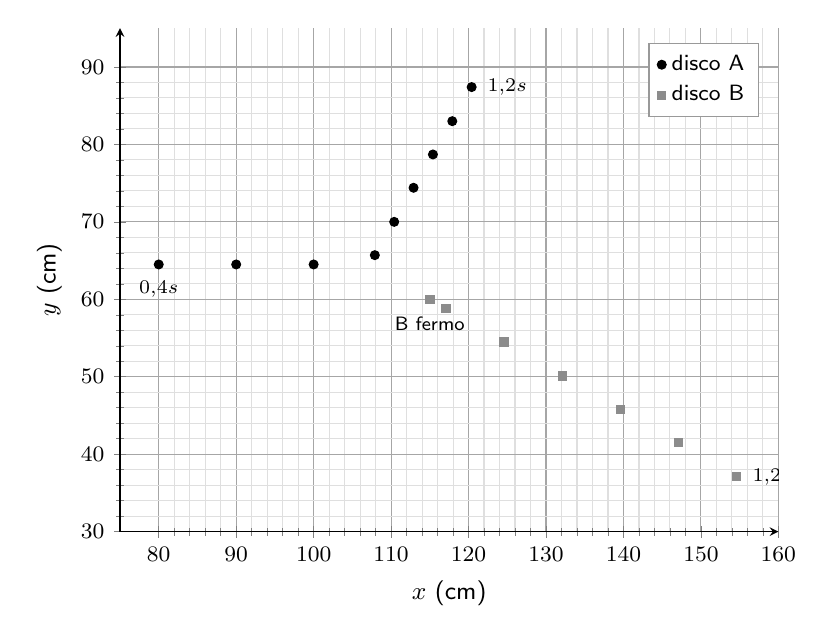
\begin{tikzpicture}
\begin{axis}[dati, axis equal image, width=.82\linewidth,
    xmin=75, xmax=160, ymin=30, ymax=95,
    xtick={80,90,...,160}, ytick={30,40,...,90}, minor tick num=4,
    xlabel={$x$ (cm)}, ylabel={$y$ (cm)}, legend pos=north east]
  \addplot[puntoA] coordinates {(80.0,64.5) (90.0,64.5) (100.0,64.5) (107.9,65.7) (110.4,70.0)
    (112.9,74.4) (115.4,78.7) (117.9,83.0) (120.4,87.4)};
  \addlegendentry{disco A}
  \addplot[puntoB] coordinates {(115.0,60.0) (117.1,58.8) (124.6,54.5) (132.1,50.1) (139.6,45.8)
    (147.1,41.5) (154.6,37.1)};
  \addlegendentry{disco B}
  \node[font=\scriptsize, anchor=north] at (axis cs:80,63.6) {$0{,}4\unm{s}$};
  \node[font=\scriptsize, anchor=west] at (axis cs:121.2,87.4) {$1{,}2\unm{s}$};
  \node[font=\scriptsize, anchor=north] at (axis cs:115,59) {B fermo};
  \node[font=\scriptsize, anchor=west] at (axis cs:155.4,37.1) {$1{,}2\unm{s}$};
\end{axis}
\end{tikzpicture}
\end{center}

\conqr{p=urti/s10\&tab=2}{%
\begin{parts}
  \itemx Dopo l'urto i due dischi partono ad angolo retto. È un caso? Verificalo con i dati, poi
    prova a spiegarlo partendo dalla quantità di moto, componente per componente, e dall'energia.
  \itemx Con l'app cambia il punto d'impatto e le masse: quando l'angolo smette di essere retto?
\end{parts}}

\begin{solution}
\textbf{a.} Prima: A a $1{,}00\unm{m/s}$ lungo $x$ ($10\unm{cm}$ ogni $0{,}1\unm{s}$). Dopo (punti
da $0{,}8$ a $1{,}2\unm{s}$): A $(0{,}25;\ 0{,}435)\unm{m/s}$, inclinata di $+60^\circ$;
B $(0{,}75;\ -0{,}435)\unm{m/s}$, inclinata di $-30^\circ$. L'angolo fra le traiettorie è
$90^\circ$. Componente $x$: $0{,}25 = 0{,}0625 + 0{,}1875\unm{kg\,m/s}$; componente $y$:
$0 = 0{,}109 - 0{,}109\unm{kg\,m/s}$. Energia: $0{,}125\unm{J}$ prima,
$0{,}031 + 0{,}094 = 0{,}125\unm{J}$ dopo, quindi l'urto è elastico.
Spiegazione: con masse uguali $\vec p_A = \vec p_A\,' + \vec p_B\,'$ è un triangolo di vettori;
la conservazione dell'energia, divisa per $m/2$, dà $p_A^2 = p_A'^2 + p_B'^2$. Per l'inverso del
teorema di Pitagora il triangolo è rettangolo.

\textbf{b.} L'angolo resta retto per ogni punto d'impatto (tranne l'urto frontale) solo con masse
uguali e urto elastico. Se A è più pesante l'angolo è minore di $90^\circ$, se è più leggero è
maggiore; con un urto anelastico è minore. Spunto facoltativo, non nel testo: nelle fotografie in camera a nebbia una particella $\alpha$ su
un nucleo di elio (masse uguali) lascia una traccia a «Y» ad angolo retto, segno di urto elastico. Le fotografie sono nella Nobel
Lecture di P.\,M.\,S. Blackett (1948), figure 1--3, con urti su ossigeno, idrogeno ed elio:
\url{https://nobelprize.org/uploads/2018/06/blackett-lecture.pdf}.
\end{solution}

\end{document}
"
\usepackage[subject=physics, seed=2026]{fancytests}
\usepackage{lmodern}
\renewcommand*\familydefault{\sfdefault}
\usepackage[T1]{fontenc}
\usepackage{qrcode}
\usepackage{url}

\geometry{a4paper, top=15mm, bottom=15mm, left=17.5mm, right=17.5mm}
\pagestyle{empty}
\linespread{1.12}

\testsetup{labels=boxed, mcq=none, autoclose=false, scores=false}

%% ---------------------------------------------------------------------------
%% QR verso una scena di Collision Lab: testo a sinistra, QR a destra
%% \conqr{frammento dopo #, con \& al posto di &}{testo}
%% ---------------------------------------------------------------------------
\newcommand{\appurl}{https://labs.matephis.com/collision-lab/}
\newcommand{\conqr}[2]{%
  \par\smallskip\noindent
  \begin{minipage}[c]{\dimexpr\linewidth-3.1cm}#2\end{minipage}\hfill
  \begin{minipage}[c]{2.6cm}\centering
    \qrcode[height=2.4cm]{\appurl\##1}\par
    {\scriptsize\color{black!55}Collision Lab}
  \end{minipage}\par\smallskip}

%% grafici di dati: assi a sinistra, griglia fitta, punti senza linee
\pgfplotsset{
  dati/.style={
    axis lines=left, grid=both, grid style={gray!70}, minor grid style={gray!25},
    tick label style={font=\footnotesize}, label style={font=\small},
    legend style={font=\footnotesize, draw=black!40, fill=white},
    legend cell align=left,
  },
  puntoA/.style={only marks, mark=*, mark size=1.6pt, black},
  puntoB/.style={only marks, mark=square*, mark size=1.5pt, black!45},
}

\begin{document}

\noindent{\Large\bfseries Fisica \textperiodcentered{} Urti in laboratorio}\par
\vspace{.4em}\noindent{\color{black!45}\rule{\textwidth}{.4pt}}\par\vspace{.4em}

\noindent Dove c'è un QR, la scena si apre in una web app. Le foto stroboscopiche sono scattate a intervalli di $0{,}1\unm{s}$.\par

\begin{solution}[Indicazioni per il docente]
\textbf{Obiettivo.} Quattro urti che coprono i casi principali: anelastico con dissipazione di
energia e moto del centro di massa (es.~1), elastico tra masse diverse nel riferimento del centro
di massa, con impulso e terzo principio (es.~2), completamente anelastico con quantità di moto
totale nulla ed elastico con un corpo che si ferma (es.~3), elastico in due dimensioni (es.~4).
Restano fuori le esplosioni.

\textbf{Struttura.} Ogni esercizio cambia punto di partenza e di arrivo, perché gli studenti non
applichino una procedura fissa: dati $\to$ energia dissipata e centro di massa (1); descrizione
$\to$ grafico previsto, calcolo, verifica (2); obiettivo $\to$ progetto della scena, verifica (3);
osservazione $\to$ spiegazione (4). Negli esercizi 2 e 3 l'app serve solo alla fine, per
controllare le risposte già date. Le domande sono aperte; conviene pretendere che ogni risposta
sia giustificata con almeno una rappresentazione.

\textbf{Tempi.} Circa un'ora: 10--15 minuti per esercizio, di più per il 3 e il 4. In
alternativa, i gruppi svolgono esercizi diversi e poi li presentano.

\textbf{Dati.} I grafici degli esercizi 1 e 4 sono stati generati con Collision Lab (stesse
masse e velocità), arrotondati al millimetro, senza rumore. Nei fotogrammi in cui i corpi sono a
contatto (es.~1, $t = 0{,}6$--$0{,}7\unm{s}$) i punti non stanno sulle rette: le velocità vanno
ricavate da punti lontani dall'urto. Nell'es.~1, $x_A$ e $x_B$ sono le estremità che si toccano,
quindi all'urto $x_A \approx x_B$.

\textbf{QR.} Es.~2: scena bloccata, aperta sul grafico $x$--$t$, con bilancio e valori numerici
nascosti; dopo previsione e calcoli, il pulsante \emph{Mostra} li rivela. Es.~3: si apre sulla
scheda \emph{Imposta}, con il velcro attivo e i vettori della quantità di moto; per verificare la
domanda b si toglie il velcro. Es.~4: preset \texttt{urti/s10}, sulla scheda \emph{Imposta}, per
cambiare masse e parametro d'urto. Nell'app il corpo A sta sempre a sinistra.
\end{solution}

%% =========================================================================
\exercise[Slitte con respingente di gomma]
Su una rotaia a cuscino d'aria orizzontale, la slitta A ($250\unm{g}$) viene spinta contro la
slitta B ($250\unm{g}$), ferma. Sul muso di A è montato un respingente ad anello di gomma. Il
grafico riporta le posizioni ricavate dal video con Tracker, ogni $0{,}1\unm{s}$: $x_A$ è la
posizione del respingente di A, $x_B$ quella del retro di B.

\begin{center}
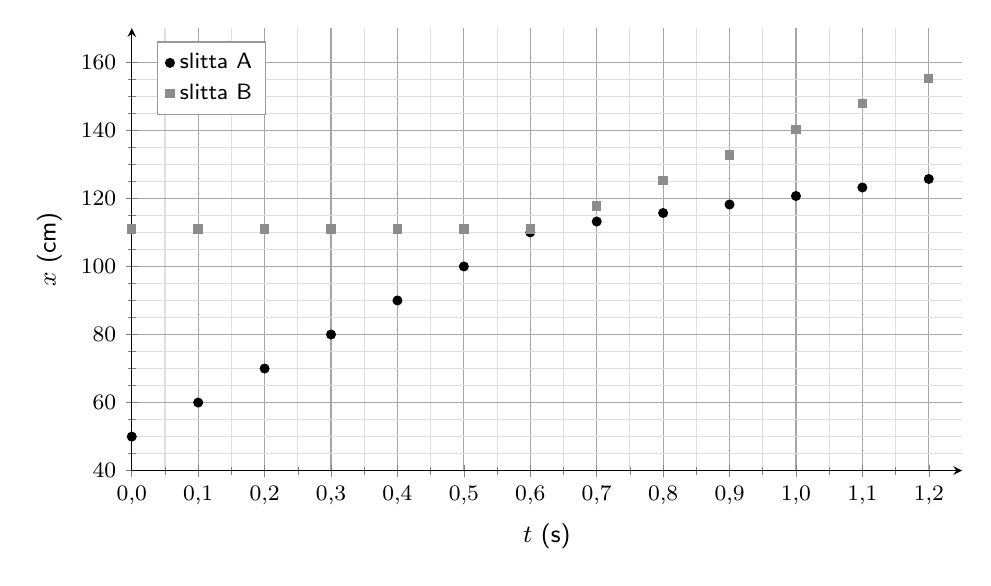
\begin{tikzpicture}
\begin{axis}[dati, width=\linewidth, height=7.2cm,
    xmin=0, xmax=1.25, ymin=40, ymax=170,
    xtick={0,0.1,...,1.2}, minor x tick num=1,
    ytick={40,60,...,160}, minor y tick num=3,
    xticklabel={\pgfmathprintnumber[fixed, fixed zerofill, precision=1, use comma]{\tick}},
    xlabel={$t$ (s)}, ylabel={$x$ (cm)}, legend pos=north west]
  \addplot[puntoA] coordinates {(0,50.0) (0.1,60.0) (0.2,70.0) (0.3,80.0) (0.4,90.0) (0.5,100.0)
    (0.6,110.0) (0.7,113.2) (0.8,115.7) (0.9,118.2) (1.0,120.7) (1.1,123.2) (1.2,125.7)};
  \addlegendentry{slitta A}
  \addplot[puntoB] coordinates {(0,111.0) (0.1,111.0) (0.2,111.0) (0.3,111.0) (0.4,111.0) (0.5,111.0)
    (0.6,111.0) (0.7,117.8) (0.8,125.3) (0.9,132.8) (1.0,140.3) (1.1,147.8) (1.2,155.3)};
  \addlegendentry{slitta B}
\end{axis}
\end{tikzpicture}
\end{center}

\begin{parts}
  \itemx Calcola la percentuale dell'energia cinetica iniziale che viene dissipata nell'urto.
  \itemx Le due slitte sono identiche. Ricava l'equazione oraria del centro di massa del sistema
    formato dalle due slitte, prima e dopo l'urto. Che cosa noti? Che legame c'è con la quantità di
    moto totale?
  \itemx Se al posto della gomma ci fosse stato un respingente di plastilina, che resta attaccato,
    come sarebbe cambiato il grafico $x$--$t$?
\end{parts}

\begin{solution}
Verso positivo verso destra. Dalle pendenze: prima $v_A = 1{,}00\unm{m/s}$, $v_B = 0$; dopo
(punti da $0{,}8$ a $1{,}2\unm{s}$) $v_A' = 10{,}0\unm{cm}/0{,}4\unm{s} = 0{,}25\unm{m/s}$ e
$v_B' = 30{,}0\unm{cm}/0{,}4\unm{s} = 0{,}75\unm{m/s}$.
Quantità di moto: $0{,}25\unm{kg\,m/s}$ prima e $0{,}0625 + 0{,}1875 = 0{,}25\unm{kg\,m/s}$
dopo.

\textbf{a.} Energia cinetica: $K_i = \tfrac12\,0{,}25\cdot 1{,}00^2 = 0{,}125\unm{J}$,
$K_f = \tfrac12\,0{,}25\,(0{,}25^2 + 0{,}75^2) = 0{,}078\unm{J}$. Dissipata:
$\dfrac{K_i - K_f}{K_i} = \dfrac{0{,}047}{0{,}125} = 37{,}5\%$ (gomma deformata e scaldata,
suono, vibrazioni). Urto anelastico: la velocità relativa passa da $1{,}00$ a $0{,}50\unm{m/s}$.

\textbf{b.} Le slitte sono identiche (lunghezza $L$): i centri stanno in $x_A - L/2$ e
$x_B + L/2$, quindi il centro di massa coincide con il punto medio dei due segni misurati,
$x_{CM} = (x_A + x_B)/2$. Dai dati: $80{,}5\unm{cm}$ a $t = 0$, $110{,}5\unm{cm}$ a $0{,}6\unm{s}$,
$140{,}5\unm{cm}$ a $1{,}2\unm{s}$, e i punti stanno sulla stessa retta anche durante l'urto:
\[ x_{CM}(t) = 0{,}805\unm{m} + (0{,}50\unm{m/s})\,t \]
prima e dopo l'urto. Il centro di massa si muove di moto rettilineo uniforme e non «si accorge»
dell'urto. La sua velocità è $v_{CM} = P/(m_A + m_B) = 0{,}25/0{,}50 = 0{,}50\unm{m/s}$: si
conserva perché si conserva la quantità di moto totale. Se gli studenti non hanno ancora visto il
centro di massa, basta la definizione $x_{CM} = (m_A x_A + m_B x_B)/(m_A + m_B)$ applicata ai centri.

\textbf{c.} Con la plastilina, dopo l'urto i due punti avanzano insieme a distanza costante:
un'unica retta (due rette parallele vicinissime) di pendenza $0{,}25/0{,}50 = 0{,}50\unm{m/s}$,
la stessa del centro di massa. L'energia cinetica finale sarebbe $0{,}0625\unm{J}$: se ne perde
metà ($50\%$).
\end{solution}

%% =========================================================================
\exercise[Slitte con magneti]
Sulla stessa rotaia, una slitta grande caricata con pesi ($500\unm{g}$ in tutto) viene lanciata a
$1{,}0\unm{m/s}$ contro una slitta piccola ($100\unm{g}$), ferma. Sulle due slitte sono montati
magneti che si respingono: le slitte non si toccano e l'urto è quasi elastico.
\medskip
\conqr{s=headon\&m1=0.5\&m2=0.1\&show=strobe\&tab=1\&g=x\&hide=bal,num\&lock=1}{%
\begin{parts}
  \itemx Senza fare calcoli, disegna il grafico $x$--$t$ che ti aspetti per le due slitte.
  \itemx Calcola la velocità del centro di massa, le velocità delle due slitte rispetto al centro
    di massa prima e dopo l'urto, e le velocità finali rispetto al laboratorio.
  \itemx Un compagno dice: «La slitta grande è cinque volte più pesante, quindi spinge la piccola
    molto più forte di quanto la piccola spinga lei». Ha ragione? Giustifica la risposta.
  \itemx Verifica con l'app (QR): confronta la foto stroboscopica con il grafico previsto e con le
    velocità calcolate, e correggi ciò che non torna.
\end{parts}}

\begin{solution}
\textbf{a.} Previsione attesa: la slitta grande rallenta ma prosegue, la piccola parte più veloce
di quanto andasse la grande. Nel grafico $x$--$t$ la retta della grande si piega verso una
pendenza minore, quella della piccola parte più ripida. Errori frequenti: la grande che si ferma
(come con masse uguali), la piccola più lenta della grande.

\textbf{b.} $v_{CM} = \dfrac{0{,}5\cdot 1{,}0}{0{,}6} = 0{,}83\unm{m/s}$. Rispetto al centro di
massa, prima: grande $1{,}0 - 0{,}83 = +0{,}17\unm{m/s}$, piccola $0 - 0{,}83 = -0{,}83\unm{m/s}$
(quantità di moto totale nulla: $0{,}5\cdot 0{,}17 - 0{,}1\cdot 0{,}83 = 0$). Nell'urto elastico le
velocità rispetto al centro di massa si invertono: dopo, grande $-0{,}17\unm{m/s}$, piccola
$+0{,}83\unm{m/s}$. Rispetto al laboratorio si somma $v_{CM}$: $v_g' = 0{,}83 - 0{,}17 =
0{,}67\unm{m/s}$, $v_p' = 0{,}83 + 0{,}83 = 1{,}67\unm{m/s}$. Stesso risultato delle formule
$v_g' = \frac{m_g - m_p}{m_g + m_p}\,v$ e $v_p' = \frac{2m_g}{m_g + m_p}\,v$.

\textbf{c.} No. Impulso sulla piccola: $0{,}1 \cdot 1{,}67 = +0{,}167\unm{N\,s}$; sulla grande:
$0{,}5\,(0{,}67 - 1{,}00) = -0{,}167\unm{N\,s}$. Per il terzo principio le forze sono uguali e
opposte e agiscono per lo stesso tempo, quindi gli impulsi sono uguali e opposti. Sono diverse
le variazioni di velocità, $\Delta v = J/m$: $-0{,}33\unm{m/s}$ per la grande, $+1{,}67\unm{m/s}$
per la piccola. È la misconcezione della dominanza: conviene far scrivere la risposta prima di
aprire la scena.

\textbf{d.} Il grafico dell'app deve mostrare la grande con pendenza $0{,}67\unm{m/s}$ e la
piccola con $1{,}67\unm{m/s}$; il pulsante \emph{Mostra} rivela bilancio e valori numerici.
\end{solution}

%% =========================================================================
\exercise[Carrelli con velcro e magneti]
Come per gli esperimenti effettuati in laboratorio, due sensori di posizione, ai due estremi della
rotaia, registrano il moto di due carrelli. Da un lato i carrelli hanno il velcro, dall'altro
magneti che si respingono. Il carrello A ha una massa aggiuntiva ($500\unm{g}$ in tutto), il
carrello B è scarico ($250\unm{g}$).
\medskip
\conqr{s=headon\&m1=0.5\&v1=0.5\&x2=1.4\&st=1\&show=strobe,mom\&tab=2}{%
\begin{parts}
  \itemx Con i lati a velcro affacciati: come vanno lanciati i due carrelli perché, dopo l'urto,
    restino fermi? Motiva la risposta.
  \itemx Ora i carrelli sono girati, con i magneti affacciati (urto quasi elastico). Si può fare in
    modo che dopo l'urto si fermi uno solo dei due? Trova almeno una soluzione e motivala.
  \itemx Verifica con l'app (QR) le risposte alle due domande precedenti; per la seconda togli il
    velcro.
\end{parts}}

\begin{solution}
\textbf{a.} I carrelli restano fermi se la quantità di moto totale è nulla:
$m_A v_A + m_B v_B = 0$, cioè $v_B = -2\,v_A$ (lanciati uno contro l'altro, B con velocità
doppia ma massa metà); per esempio $v_A = +0{,}25\unm{m/s}$ e $v_B = -0{,}50\unm{m/s}$. La
motivazione è la conservazione della quantità di moto: se prima le due quantità di moto sono
uguali e opposte (somma nulla) e i carrelli restano attaccati, dopo la somma è nulla solo se la
velocità comune è nulla. Con il diagramma a barre: prima due barre di uguale lunghezza e verso
opposto, dopo nessuna barra. L'energia cinetica
($0{,}016 + 0{,}031 = 0{,}047\unm{J}$ nell'esempio) sparisce tutta: è l'unico caso in cui un urto
la fa sparire tutta.

\textbf{b.} Con l'urto elastico si può fermare A. Le condizioni sono la conservazione della
quantità di moto e l'inversione della velocità relativa ($v_B' - v_A' = v_A - v_B$); con
$v_A' = 0$ si ottiene $v_B = -0{,}5\,v_A$. Per esempio $v_A = +0{,}60\unm{m/s}$,
$v_B = -0{,}30\unm{m/s}$: dopo l'urto A è fermo e B riparte a $+0{,}90\unm{m/s}$. Con B fermo
all'inizio non si riesce (servirebbero masse uguali). Fermare B è impossibile: B dovrebbe
allontanarsi da A più veloce di lui, e l'urto non avverrebbe.

\textbf{c.} Per la a basta la scena così com'è (velcro attivo) con $v_A$ e $v_B$ nel rapporto
trovato; per la b si toglie il velcro e si impostano le velocità. Sulla rotaia vera i magneti non
danno un urto perfettamente elastico e c'è un po' di attrito: A non si fermerebbe del tutto, e
questo è un buon punto di discussione, ma non è richiesto di provarlo.
\end{solution}

%% =========================================================================
\newpage
\exercise[Dischi sul tavolo a cuscino d'aria]
Su un tavolo a cuscino d'aria orizzontale, il disco A ($250\unm{g}$, diametro $9\unm{cm}$)
colpisce di striscio il disco B, identico e fermo. I bordi dei dischi sono rivestiti da un anello
elastico. Lo smartphone, fissato sopra il tavolo, riprende la scena; il grafico riporta le
posizioni dei centri ricavate con Tracker, ogni $0{,}1\unm{s}$, da $t = 0{,}4\unm{s}$ a
$t = 1{,}2\unm{s}$.

\begin{center}
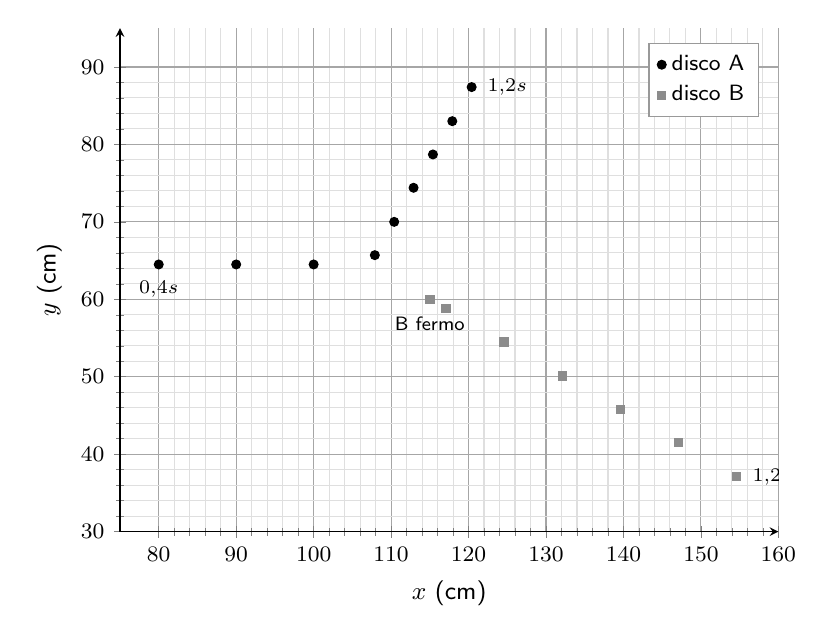
\begin{tikzpicture}
\begin{axis}[dati, axis equal image, width=.82\linewidth,
    xmin=75, xmax=160, ymin=30, ymax=95,
    xtick={80,90,...,160}, ytick={30,40,...,90}, minor tick num=4,
    xlabel={$x$ (cm)}, ylabel={$y$ (cm)}, legend pos=north east]
  \addplot[puntoA] coordinates {(80.0,64.5) (90.0,64.5) (100.0,64.5) (107.9,65.7) (110.4,70.0)
    (112.9,74.4) (115.4,78.7) (117.9,83.0) (120.4,87.4)};
  \addlegendentry{disco A}
  \addplot[puntoB] coordinates {(115.0,60.0) (117.1,58.8) (124.6,54.5) (132.1,50.1) (139.6,45.8)
    (147.1,41.5) (154.6,37.1)};
  \addlegendentry{disco B}
  \node[font=\scriptsize, anchor=north] at (axis cs:80,63.6) {$0{,}4\unm{s}$};
  \node[font=\scriptsize, anchor=west] at (axis cs:121.2,87.4) {$1{,}2\unm{s}$};
  \node[font=\scriptsize, anchor=north] at (axis cs:115,59) {B fermo};
  \node[font=\scriptsize, anchor=west] at (axis cs:155.4,37.1) {$1{,}2\unm{s}$};
\end{axis}
\end{tikzpicture}
\end{center}

\conqr{p=urti/s10\&tab=2}{%
\begin{parts}
  \itemx Dopo l'urto i due dischi partono ad angolo retto. È un caso? Verificalo con i dati, poi
    prova a spiegarlo partendo dalla quantità di moto, componente per componente, e dall'energia.
  \itemx Con l'app cambia il punto d'impatto e le masse: quando l'angolo smette di essere retto?
\end{parts}}

\begin{solution}
\textbf{a.} Prima: A a $1{,}00\unm{m/s}$ lungo $x$ ($10\unm{cm}$ ogni $0{,}1\unm{s}$). Dopo (punti
da $0{,}8$ a $1{,}2\unm{s}$): A $(0{,}25;\ 0{,}435)\unm{m/s}$, inclinata di $+60^\circ$;
B $(0{,}75;\ -0{,}435)\unm{m/s}$, inclinata di $-30^\circ$. L'angolo fra le traiettorie è
$90^\circ$. Componente $x$: $0{,}25 = 0{,}0625 + 0{,}1875\unm{kg\,m/s}$; componente $y$:
$0 = 0{,}109 - 0{,}109\unm{kg\,m/s}$. Energia: $0{,}125\unm{J}$ prima,
$0{,}031 + 0{,}094 = 0{,}125\unm{J}$ dopo, quindi l'urto è elastico.
Spiegazione: con masse uguali $\vec p_A = \vec p_A\,' + \vec p_B\,'$ è un triangolo di vettori;
la conservazione dell'energia, divisa per $m/2$, dà $p_A^2 = p_A'^2 + p_B'^2$. Per l'inverso del
teorema di Pitagora il triangolo è rettangolo.

\textbf{b.} L'angolo resta retto per ogni punto d'impatto (tranne l'urto frontale) solo con masse
uguali e urto elastico. Se A è più pesante l'angolo è minore di $90^\circ$, se è più leggero è
maggiore; con un urto anelastico è minore. Spunto facoltativo, non nel testo: nelle fotografie in camera a nebbia una particella $\alpha$ su
un nucleo di elio (masse uguali) lascia una traccia a «Y» ad angolo retto, segno di urto elastico. Le fotografie sono nella Nobel
Lecture di P.\,M.\,S. Blackett (1948), figure 1--3, con urti su ossigeno, idrogeno ed elio:
\url{https://nobelprize.org/uploads/2018/06/blackett-lecture.pdf}.
\end{solution}

\end{document}
